% IN THIS SECTION SHOW SOME OF OUR TRANSLATED CODE... AND WALK THROUGH IT THE SAME WAY YOU DID WITH THE CONCEPT IN RESOLVE. BUT BEFORE YOU DO THAT, SHOW THE PICTURE (The one thats already here showing high level relationships and update it!).
\section{Implementation}
Development of our C translation tool can be logically partitioned into three distinct phases: 
\begin{enumerate}
\item Arriving at a translation model (or, strategy) for an accurate C representation of RESOLVE.
\item Implementing reusable mechanisms for carrying out the C code generation process.
\item Creation of a memory manager capable of safely allocating and freeing dynamic memory required by the generated code.
\end{enumerate}
We conclude this section with a demonstration of each of these phases working in tandem on the LED component discussed in Section \ref{sec:specifiying}. 

\subsection{C Translation Model}
One of the primary challenges in translating from RESOLVE to C is finding a suitable C analog for each RESOLVE module and the constructs allowable in each. Indeed, since we are dealing with an environment where functional correctness is a primary concern, it is important that the code generated by our tool represents as closely as possible the original RESOLVE source. In an effort to make such considerations, at the highest level, the C code we generate makes special considerations for concepts, facilities, and realizations. This scheme is depicted in Figure \ref{fig:relationship} and briefly summarized in Sections \ref{sec:conceptoverview} - \ref{sec:facilitiesrealizations}.

\begin{figure}
\begin{center}
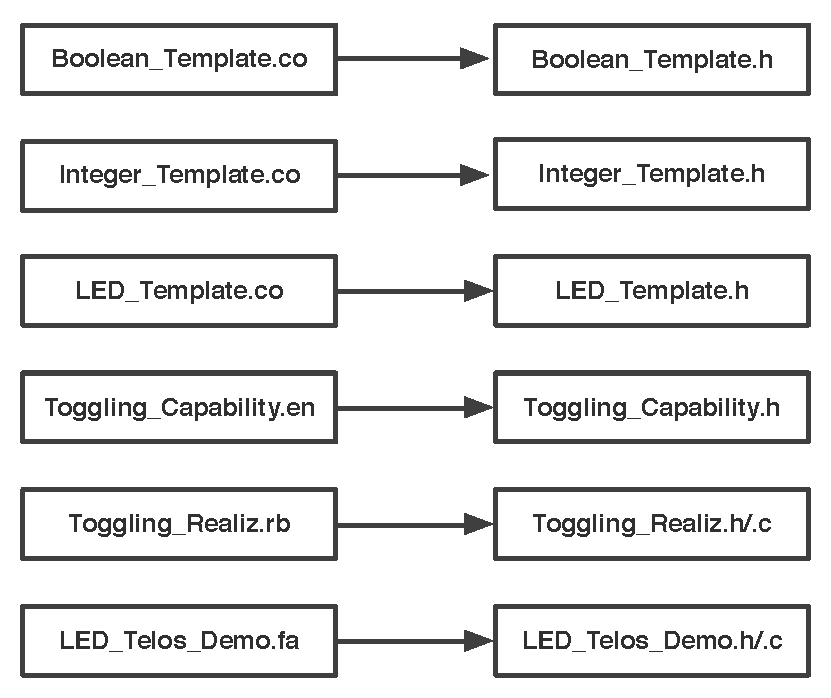
\includegraphics[scale=.60]{figs/relationship.pdf}
\end{center}
\caption{Relationship between RESOLVE module types and the C code generated from each.}
\label{fig:relationship}
\end{figure}

\subsubsection{Concepts}
\label{sec:conceptoverview}
Concept modules produce a single .h file, which provide function pointers for the operations specified in the original concept, as well as structs representing each user defined type. 

\subsubsection{Facilities}
\label{sec:facilitiesoverview}
Facilities produce an .h/.c pair: The header .h declares both a ``create" and ``destroy" method which, taken together, encapsulates the creation and destruction of all global variables used within the facility. The .c provides an implementation of these methods.  Note that these create and destroy methods are only responsible for freeing \textit{global} variables -- meaning all other translated functions are responsible for deallocating their own local variables. 

\subsubsection{Realizations}
\label{sec:facilitiesrealizations}
We treat realizations of concepts and enhancements slightly different than facility modules. While a .h/.c pair is still produced, the create method designated in the header for realizations is designed to create instances of all types specified by the concept, while the destroy method deallocates these types -- as opposed to simply destroying user created globals.

%The memory model must also be considered as an additional verifiable component. Currently, RESOLVE is not capable of creating a complete specification of memory\footnote{RESOLVE is an object based language and has variable sized structures. Using dynamically allocatable memory is the favored approach to allow arbitrarily sized data.}. Thus, a memory model must be realized without a specification. To provide a straight forward translation from RESOLVE to C, we provide a dynamically-based memory allocator for use on embedded systems.

%Unsurprisingly, concepts are represented in C by a single header .h listing the various methods 

\begin{figure*}
\begin{center}
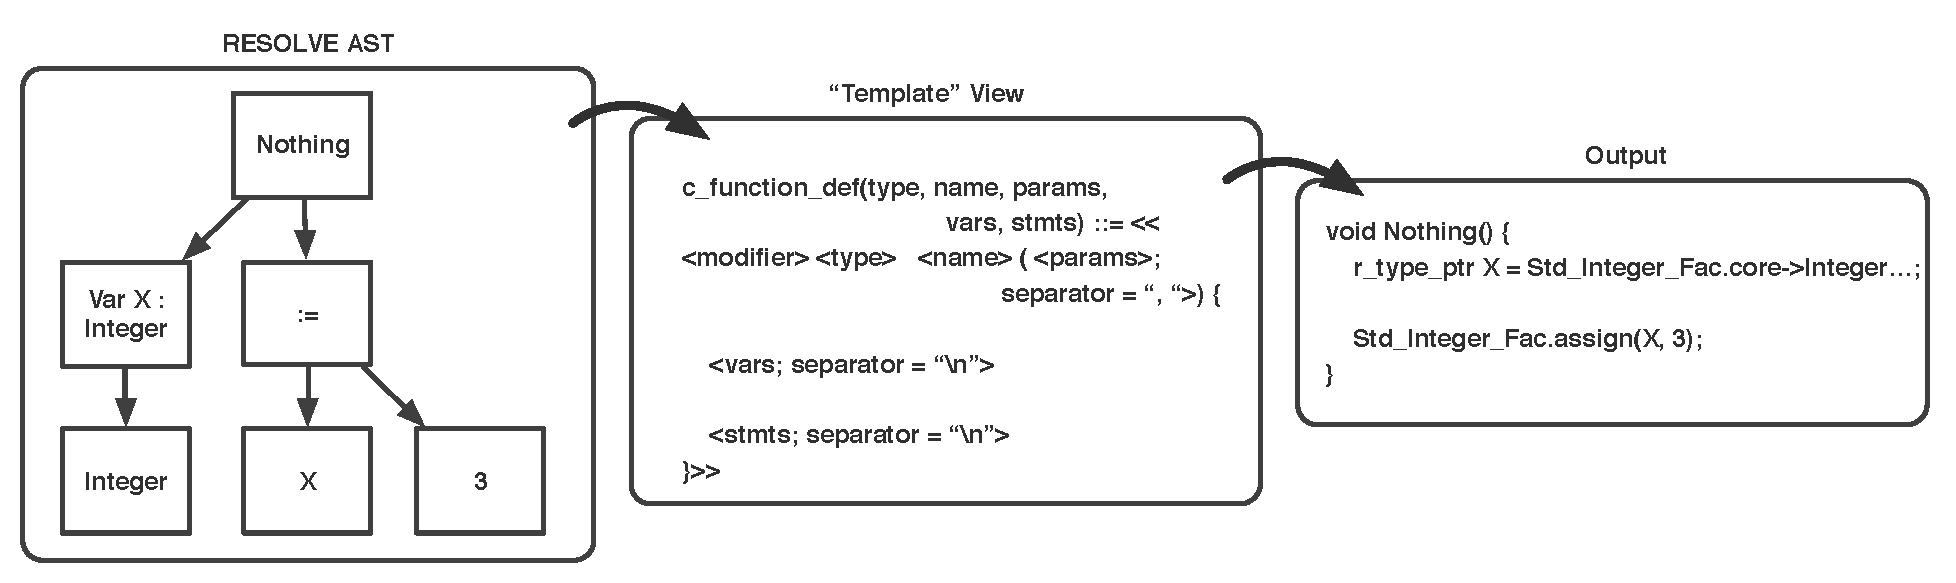
\includegraphics[scale=.55]{figs/ast_traversal2.pdf}
\end{center}
\caption{The general flow of information from the AST (first), to user defined templates (middle), ending with formed output (last).}
\label{fig:ast}
\end{figure*}


\subsection{Translator Implementation}

Translation itself occurs over the course of a traversal of RESOLVE's abstract syntax tree (AST) -- an intermediate representation of RESOLVE code. The traversal mechanism utilized is a derivative of the visitor pattern that provides a pre post traversal over all nodes in the tree. 

%\subsubsection{AST Traversal}
%Translation is performed over the course of a traversal of RESOLVE's abstract syntax tree (AST). The traversal mechanism used is a dervivative of the visitor pattern that provides a SAX-dom style pre-post traversal over all nodes in the tree. Thus, for any given node present, a total of two visits occur: One corresponding to the node being `hit' during the pre traversal stage, and one for the post. 

To illustrate the general process of producing runnable C from RESOLVE code, consider the following dummy operation:

\begin{verbatim}
Operation Nothing(); Procedure
        Var X : Integer;
        X := 3;
end Nothing;
\end{verbatim}

Shown in Figure \ref{fig:ast} is a high level depiction of steps taken in translating this operation to C. The first box depicts the AST of \texttt{Nothing}, where nodes are represented with boxes labeled by the constructs they contain. Throughout the walk of this tree, useful information (such as the operation's name, ``Nothing") are extracted from the nodes containing these constructs, and added to a user defined string-template\footnote{A template can simply be thought of as a ``document with holes" which the user choses when and how to fill.}, in this case: \texttt{c\_function\_def}.

In the context of RESOLVE to C translation, these templates, when filled during the aforementioned pre-post visitor traversal of RESOLVE's AST, help simplify the task of producing complicated, arbitrarily nested blocks of structured C output by keeping translation logic strictly within the C translator, and output logic strictly within the templates.

That is, the only actual work being performed within the C translator is forwarding information gathered from individual treenodes, to a series of externally defined templates. This allows us to exploit (in design pattern parlance) a strict model view controller (MVC) separation in the translator's codebase between the mechanism that does the AST visiting (controller), the tree nodes from which we're adding information to templates (model), and the external file containing all available C language templates which shape our output (view).

We feel this approach lends itself well to the challenge discussed in this paper, as this separation allows us to easily iterate changes to our generated C code without needing to concern ourselves with the Java written inside the compiler itself. This allows us to easily and iteratively tweak generated code -- making arbitrarily complicated changes and optimizations, some of which are detailed later in Section \#.

% general flow Each of these calls are received in the translator in the order in which they are visited within the tree. It is up to the client (in this case, the author of the C-translator) to decide which of these methods they wish to override and perform custom actions within. 

%\subsubsection{Translation output}
%Output of translated code is done using \textit{Stringtemplate} -- a third-party tool written in Java that allows users to define parameterizable templates. Like the name suggests, a template is simply ``a document with holes" that the user choses when and how to fill. 

%An example C function definition template is shown below.

%\begin{verbatim}
%function_def(modifier, type, name, params, 
%                               vars, stmts) ::= <<
%<modifier> <type> <name> (<params; sep = ", ">) {
%    <vars; sep = "\n">
%    <stmts; sep = "\n">
%}>>
%\end{verbatim}

%User supplied attributes, enclosed in \texttt{<..>}, indicates the position of that attribute relative to others. It is entirely up to the user to define which attributes to fill in, and how complex they want them to be. For example, the user might choose to fill the \texttt{params} attribute with a simple string, or a separately defined \texttt{parameter} template, which in turn might use another separately defined \texttt{type} template.

%\begin{verbatim}
%parameter(type, name) ::= "<type> <name>"
%\end{verbatim}

%In the context of language translation, these templates, when stored on a stack and manipulated over the course of the aforementioned AST traversal, help simplify the task of producing complicated, structured blocks of C output. For instance, upon visiting \texttt{preOperationDec}, a \texttt{function\_def} template can be instantiated by the client and pushed onto a global translation stack with its \texttt{name}, return \texttt{type}, and \texttt{modifier} attributes filled in. As \texttt{preOperationDec}'s children are visited, the \texttt{function\_def} template currently at the top of the stack receives similarly constructed parameter, variable, and statement templates from the nodes being walked. Upon reaching \texttt{postOperationDec}, we can be assured that the function has been completely filled in with the appropriate templates -- assuming the user has implemented the children's visit methods.

%Hence, the only actual work being performed within visit methods is forwarding appropriate information from tree-node it represents, to an externally defined template. This allows us to exploit (in shameless design pattern parlance) a strict model view controller (MVC) separation in the translator's codebase between the mechanism that does the AST visiting (controller), the tree nodes from which we're adding information to templates (model), and the external file containing all available C language templates (view).

<<<<<<< HEAD
\subsection{Memory Allocation}

Any model seeking to convert RESOLVE to a lower level representation such as C demands a strategy for handling any memory utilized by the generated code. While dynamic allocation is typically the norm, it is not however the first choice for embedded applications. With the Telos mote constrained to 128 bytes of RAM, developers targeting embedded platforms tend to favor static memory allocation over dynamic, due the memory efficiency it affords. 

%Many programs however benefit greatly from dynamic memory allocation not only in terms of clarity and straightforwardness, but in our case: Accurately modeling exactly what the code being executed is doing. 
%NesC, for example, while giving the illusion of dynamic allocation, behind the scenes actually performs static allocation 

In spite of this, our reasoning for choosing to pursue dynamic allocation over static, rests in the language itself. Being a language that relies heavily on the notion of formally specified objects (components), everything in RESOLVE from the `primitive' types such as booleans and integers, to the more complicated (user defined) ones such as Stacks and Queues, are modeled, specified, and implemented in the same way: Using the standard RESOLVE machinery discussed in Section \ref{sec:specifiying}. 

=======
%%%%%%%%%%%%%%%%%%%%%%%
%           Memory Allocation Section              %
%%%%%%%%%%%%%%%%%%%%%%%
\subsection{Memory Allocation}\label{sec:mem}

Any model seeking to convert RESOLVE to a lower level representation such as C demands a strategy for handling any memory utilized by the generated code. While dynamic allocation is typically the norm, it is not however the first choice for embedded applications. With the Telos mote constrained to 128 bytes of RAM, developers targeting embedded platforms tend to favor static memory allocation over dynamic, due the memory efficiency it affords. 

%Many programs however benefit greatly from dynamic memory allocation not only in terms of clarity and straightforwardness, but in our case: Accurately modeling exactly what the code being executed is doing. 
%NesC, for example, while giving the illusion of dynamic allocation, behind the scenes actually performs static allocation 

In spite of this, our reasoning for choosing to pursue dynamic allocation over static, rests in the language itself. Being a language that relies heavily on the notion of formally specified objects (components), everything in RESOLVE from the `primitive' types such as booleans and integers, to the more complicated (user defined) ones such as Stacks and Queues, are modeled, specified, and implemented in the same way: Using the standard RESOLVE machinery discussed in Section \ref{sec:specifiying}. 

>>>>>>> bolte
As such, even the simplest RESOLVE programs still rely heavily on the notion of objects coming and going. Thus, from a verification perspective, creating a tool that allows our translated code to create and destroy such objects in the manner the language itself uses is an important component to capture in formally verified code.

\subsubsection{Allocation using \texttt{salloc}}

<<<<<<< HEAD
The particular allocation scheme that we chose to use is \texttt{salloc()}: A first fit memory allocator. Rather than allocating memory on the heap, \texttt{salloc()} instead uses the stack. At compilation, the allocator provisions a fixed size of memory. It requires a small section of meta-data called a block which contains information of about the size of memory allocated, neighboring blocks, as well if the block is free or not. A sample representation of the stack shown in figure \ref{fig:stack}, is a typical example of allocated memory on the stack.
=======
The particular allocation scheme that we chose to use is \texttt{salloc()}: A first fit memory allocator. Rather than conventional, heap-based allocators, \texttt{salloc()} uses stack memory for allocation. This approach requires that a fixed size of memory is chosen at compilation. In addition, \texttt{salloc()}, requires a section of meta-data, which is denoted as a \texttt{block}, for each record in the memory pool. A \texttt{block} holds referential information of neighboring blocks, the size of the record the block maintains, and if the block is free or is in use. Figure~\ref{fig:stack} is an example of the stack after several calls to \texttt{salloc()}.
>>>>>>> bolte

\begin{figure}[!htb]
%\centering
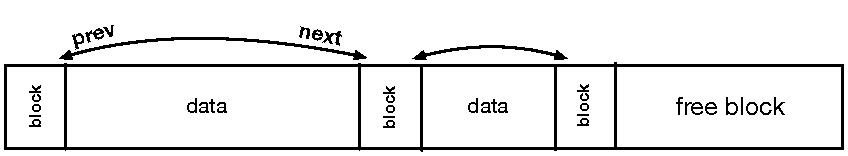
\includegraphics[scale=.55]{figs/stack.pdf}
\caption{Representation of memory using salloc()}
Memory allocated with salloc() allocates a block in front of data allocated. Blocks point to their immediate neighbors and hold their size and usage.
\label{fig:stack}
\end{figure}

\subsubsection{Deallocation using \texttt{sfree}}

A memory allocator must provide a mechanism to release, or free memory in order to indicate that it is not being used and can be reallocated. The \texttt{sfree()} function provides deallocation for memory allocated with \texttt{salloc()}. Figure~\ref{fig:free} shows an example set of memory before and after calling \texttt{sfree()}. 

\begin{figure}[!htb]
%\centering
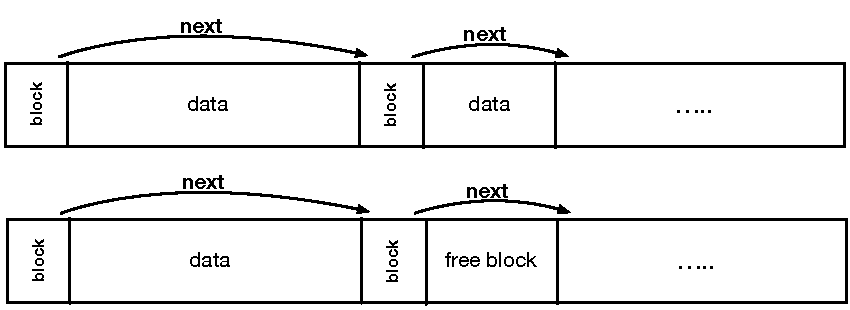
\includegraphics[scale=.55]{figs/sfree.pdf}
\caption{sfree to free memory}
\label{fig:free}
\end{figure}

\subsubsection{Optimizing Memory Usage}

A common problem that can occur in memory allocation is fragmentation. During execution, a program can allocate and deallocate an arbitrary number of times. Figure~\ref{fig:fragmentation} shows problems that result from this. This problem is magnified on embedded systems due to their limited memory capacities. There are simple optimizations that can reduce fragmentation. 

Block splitting, as shown in Figure~\ref{fig:split}, occurs during allocation. It allows blocks of greater size to be partitioned into the size requested by the allocator. 

Fusing blocks is another technique used when \texttt{sfree()} is called. When memory is deallocated, neighboring free blocks are coalesced to form a single large block, as shown in Figure~\ref{fig:fuse}. 

\begin{figure}[!htb]
\centering
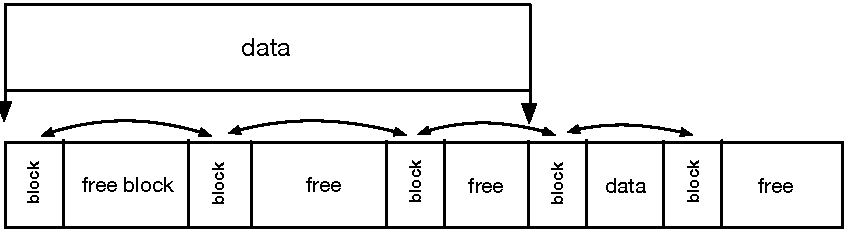
\includegraphics[scale=.55]{figs/fragmentation.pdf}
\caption{Performing naive allocation and deallocations, allocatable blocks are restricted to those that match the exact size of memory requested from the allocator}
\label{fig:fragmentation}
\end{figure}

\begin{figure}[!htb]
\centering
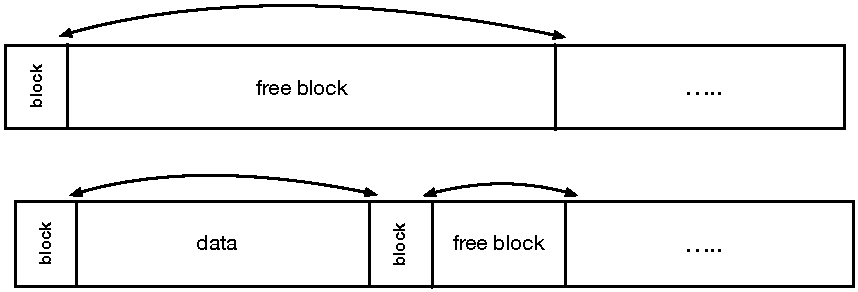
\includegraphics[scale=.55]{figs/split.pdf}
\caption{Splitting creates a block that is the size that the allocator requested, and a new free block with the remainder of memory.}
\label{fig:split}
\end{figure}


\begin{figure}[!htb]
\centering
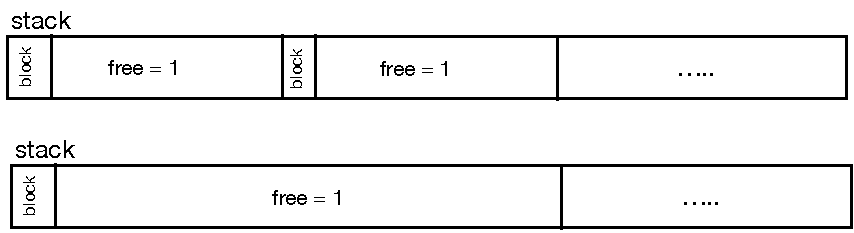
\includegraphics[scale=.55]{figs/fuse.pdf}
\caption{Block fusing. This creates single larger block, decreasing the number of smaller blocks unable to split.}
\label{fig:fuse}
\end{figure}

%
%
